%% %%%%%%%%%%%%%%%%%%%%%%%%%%%%%%%%%%%%%%%%%%%%%%%%%
%% Template for a conference paper, prepared for the
%% Food and Resource Economics Department - IFAS
%% UNIVERSITY OF FLORIDA
%% %%%%%%%%%%%%%%%%%%%%%%%%%%%%%%%%%%%%%%%%%%%%%%%%%
%% Version 1.0 // November 2019
%% %%%%%%%%%%%%%%%%%%%%%%%%%%%%%%%%%%%%%%%%%%%%%%%%%
%% Ariel Soto-Caro
%%  - asotocaro@ufl.edu
%%  - arielsotocaro@gmail.com
%% %%%%%%%%%%%%%%%%%%%%%%%%%%%%%%%%%%%%%%%%%%%%%%%%%
\documentclass[11pt]{article}
\usepackage{UF_FRED_paper_style}
\usepackage{tabularx}
\usepackage{siunitx}
\usepackage{tipa}
\usepackage{textcmds}
\usepackage{multirow} 
%\usepackage{xcolor}
\usepackage[dvipsnames]{xcolor}
\usepackage{soul}
\definecolor{HLColor}{RGB}{230,230,250}
\sethlcolor{HLColor}
\usepackage[
    backend=biber,
    style=numeric,
  ]{biblatex}

\addbibresource{references.bib}
%% ===============================================
%% Setting the line spacing (3 options: only pick one)
%\doublespacing
% \singlespacing
\onehalfspacing
%% ===============================================
 
%\setlength{\droptitle}{-5em} %% Don't touch

% %%%%%%%%%%%%%%%%%%%%%%%%%%%%%%%%%%%%%%%%%%%%%%%%%%%%%%%%%%
% SET THE TITLE
% %%%%%%%%%%%%%%%%%%%%%%%%%%%%%%%%%%%%%%%%%%%%%%%%%%%%%%%%%%

% TITLE:
\title{\textbf{User Interface Design: Deliverable D3}\\Moodtracker for Companies}

% AUTHORS:
\author{Laurenz Kottek\\ Céline Nöhl\\ Alexandros Tsaparas\\ Noé Barbera}


    
% DATE:
\date{\today}

% %%%%%%%%%%%%%%%%%%%%%%%%%%%%%%%%%%%%%%%%%%%%%%%%%%%%%%%%%%
% %%%%%%%%%%%%%%%%%%%%%%%%%%%%%%%%%%%%%%%%%%%%%%%%%%%%%%%%%%
\begin{document}
% %%%%%%%%%%%%%%%%%%%%%%%%%%%%%%%%%%%%%%%%%%%%%%%%%%%%%%%%%%
% %%%%%%%%%%%%%%%%%%%%%%%%%%%%%%%%%%%%%%%%%%%%%%%%%%%%%%%%%%
% ABSTRACT
% %%%%%%%%%%%%%%%%%%%%%%%%%%%%%%%%%%%%%%%%%%%%%%%%%%%%%%%%%%
% %%%%%%%%%%%%%%%%%%%%%%%%%%%%%%%%%%%%%%%%%%%%%%%%%%%%%%%%%%
{\setstretch{.8}}
\maketitle 

\vspace{15mm}


\tableofcontents
\newpage

\section{Introduction}
While we were creating the paper mockup for our app, it quickly became clear that our app was going to be very extensive. As we basically need two different user interfaces for team members and team leaders, we have a considerable amount of extra work. For this reason, we decided to initially develop the Lo-Fi prototype for the team leader side only. Later, we can then more easily create the interface for the team members, as we already have the basic design and fewer functions are required than for the team leaders. For this reason, the following report will only deal with the team leader side.

\section{Prototype}
The prototype is limited to a few functions of the later app. The aim is to analyse how clear and concise the design of the interface is and how easy it is for users to find their way around the app. Figma was used to create a functioning prototype with interactive parts. The complete prototype as a figma file is attached to this file. A screenshot of the prototype taken during a user test is attached as well. You can also test the prototype under this \href{https://www.figma.com/proto/eesoN637wOm4ooDvH1GrsL/Mood-Tracker?type=design&node-id=33-360&t=JI5o14rbvK1Bx76C-0&scaling=min-zoom&page-id=0%3A1&starting-point-node-id=33%3A360}{\textbf{link}}.\\
The prototype covers starting the app with an existing login, selecting a team and creating a new survey. There are already several existing teams from which the user can choose. There are also many options for creating a new survey. As we are focussing on the team leader, we cover scenarios 1 and 4 from D2. We have retained the login screen from the mockup in D2, where each user is asked to enter their daily mood. This screen is shown in Figure \ref{fig:login}.

\begin{figure}[h!]
    \centering
    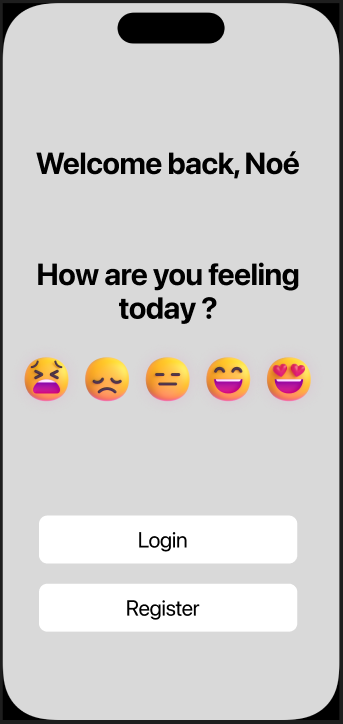
\includegraphics[width=0.3\linewidth]{figures/Login-Screen.PNG}
    \caption{Login screen of the mood tracker app.}
    \label{fig:login}
\end{figure}
Once the users have answered the question, they are redirected to the main screen (Figure \ref{fig:mainscreen}), where they can see an overview of the existing teams. If a team is selected, the user is taken to the team overview (Figure \ref{fig:teamoverview}), from where various actions can be carried out. However, due to the small extent of a Lo-Fi prototype, only the creation of a new survey and viewing the survey results were implemented here. These actions also cover the scenarios mentioned above.

\begin{figure}
     \centering
     \begin{subfigure}[b]{0.4\textwidth}
         \centering
         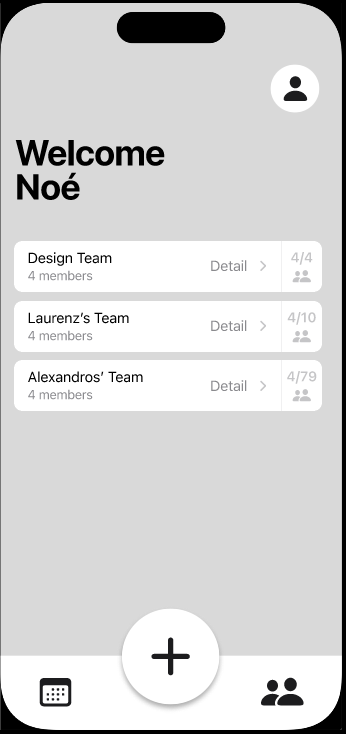
\includegraphics[width=\textwidth]{figures/Main-Screen.PNG}
         \caption{Mainscreen with the overview of all existing teams.}
         \label{fig:mainscreen}
     \end{subfigure}
     \hfill
     \begin{subfigure}[b]{0.4\textwidth}
         \centering
         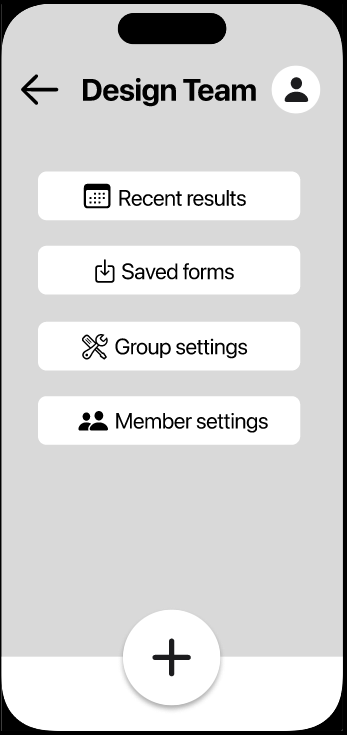
\includegraphics[width=\textwidth]{figures/Team-Overview.PNG}
         \caption{Team overview of the chosen team.\\  \mbox{}\\}
         \label{fig:teamoverview}
     \end{subfigure}
        \caption{Mainscreen and Team overview of the app.}
\end{figure}


\clearpage

\section{User Tests}
The following describes the goals of our User Tests, how we selected the participants for the tests, performed the user tests, and finally analysed them.


\subsection{Goals of the User Tests}
The goal of our User tests was primarily to find out more about the usability of our prototype focusing on the participants' ability to accomplish the given tasks within the prototype. The focus here was on creating new teams and new surveys. In addition, the design of the app was to be evaluated. These tasks were fundamental in meeting the criteria for the previously described scenarios. 

\subsection{Participants}
Our app is aimed at companies, but as this app is being designed as part of a university course, it is unfortunately not possible for us to carry out user tests with users from the right target group. Therefore, at the beginning of the test, we asked the users to put themselves in the role of a team leader in a company.\\
We also tried to keep the group as diverse as possible, but this proved to be difficult due to our almost exclusively student environment.


\subsection{Execution and Setup}
The user tests were carried out according to the Wizard of Oz Principle. However, as our prototype can already handle the most important interactions automatically, the method has been modified slightly. In addition, no artifacts were used as the app does not require any interactions with the environment.\\
First of all, the participant is given a brief introduction to our app and is handed the task sheet. If the participant has no further questions, the test can begin. Due to the space available, the participant and a member of our group (supervisor) sit next to each other, as shown in Figure \ref{fig:test setup}. The supervisor takes notes during the test. The prototype on which the tasks are to be solved can be seen on the participant's laptop. After completing the tasks, the test person fills out a short survey and is then finished, when no further questions are asked or some additional feedback is given. The information sheet with the tasks and the User Test survey are attached to the file. Figures \ref{fig:lenaUser}  and \ref{fig:setup} shows pictures of the test setup. 
\begin{figure}[h!]
    \centering
    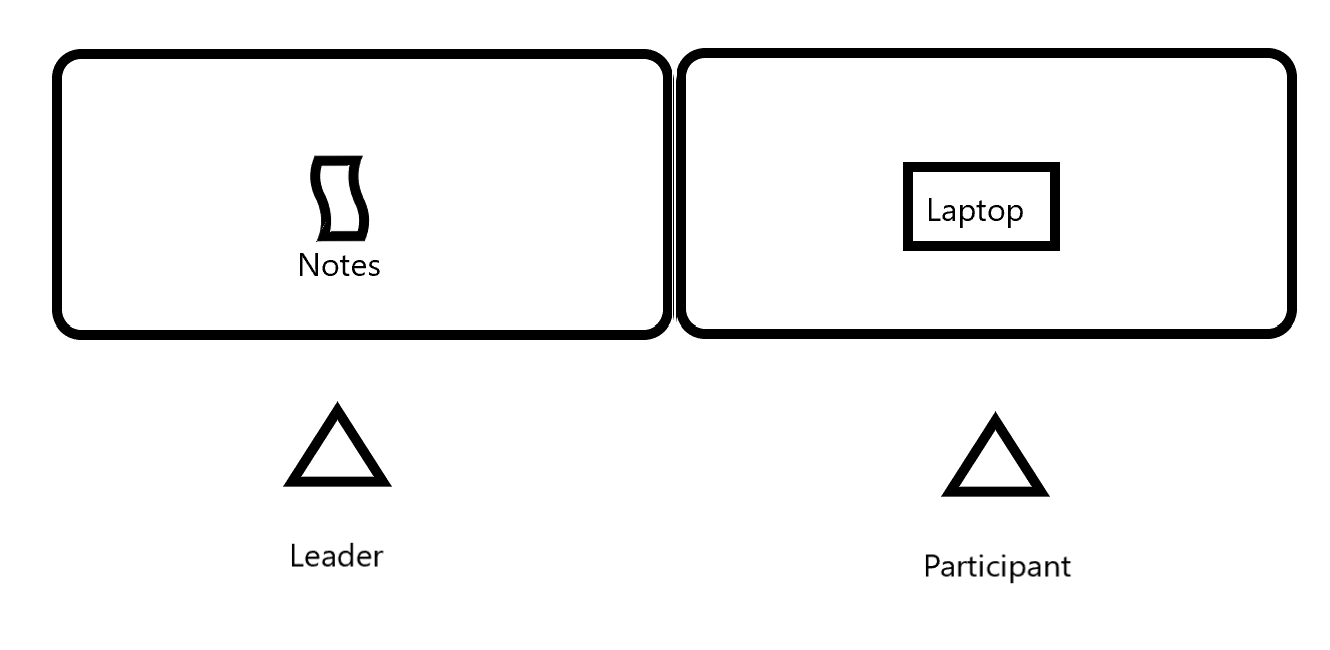
\includegraphics[width=0.8\linewidth]{figures/User Test Setup.png}
    \caption{Schematic of the structure used for the user tests.}
    \label{fig:test setup}
\end{figure}

\begin{figure}[h!]
    \begin{subfigure}[b]{0.4\textwidth}
         \centering
         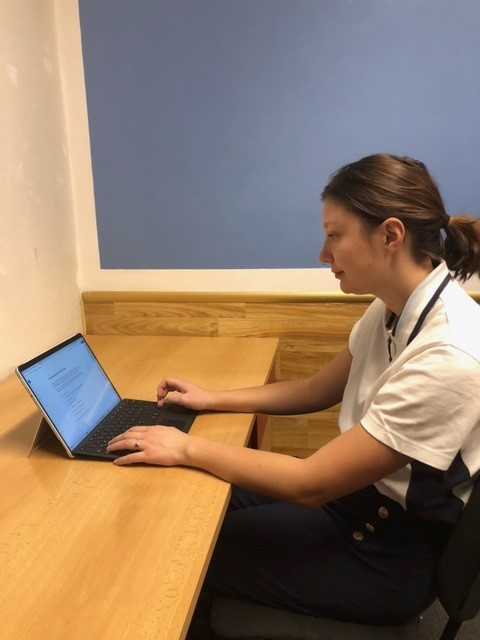
\includegraphics[width=\textwidth]{figures/Picture P1 Lena.jpg}
         \caption{A participant taking the user test in real life.}
         \label{fig:lenaUser}
    \end{subfigure}
    \hfill
    \begin{subfigure}[b]{0.53\textwidth}
         \centering
         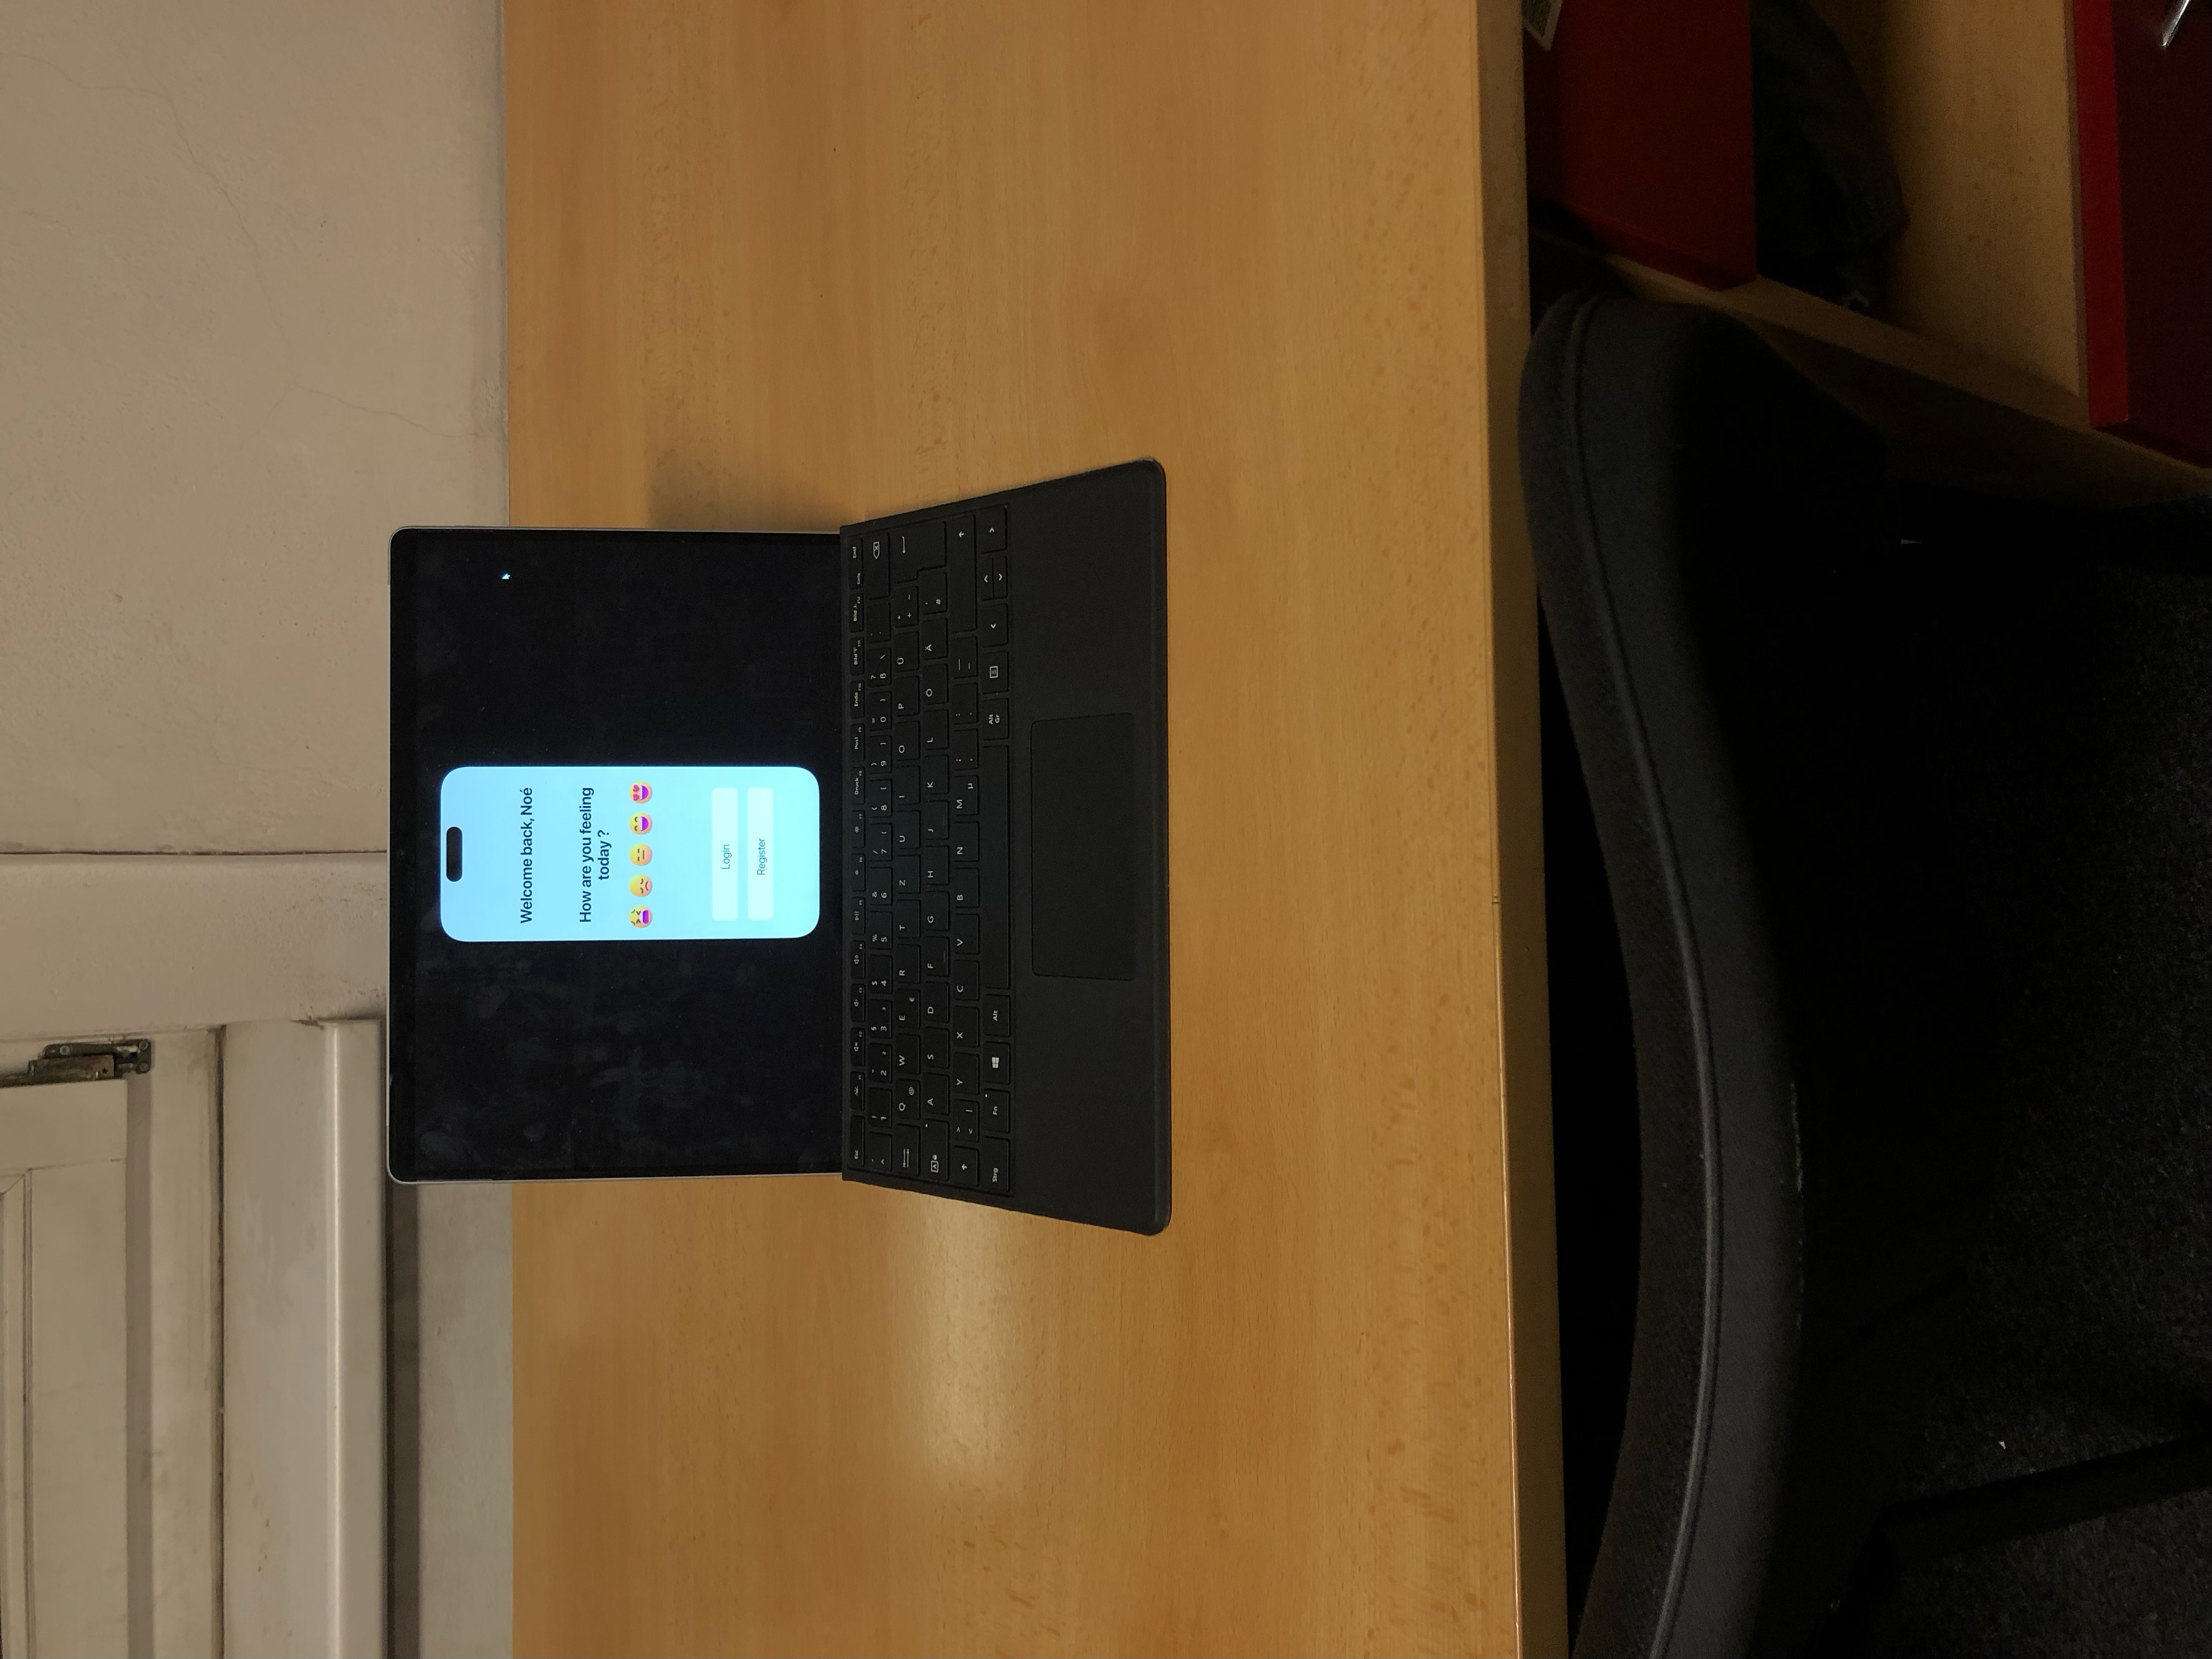
\includegraphics[width=\textwidth, angle=-90]{figures/Test Setup front.jpeg}
         \caption{The setup of the user test.}
         \label{fig:setup}
     \end{subfigure}
        \caption{Examples of the user test's setup.}
\end{figure}
\clearpage

\subsection{Evaluation}
We thought about how we wanted to analyse the user test in advance. To do this, we created a survey tailored to the tasks that the test subjects had to fulfill in order to collect feedback. The survey can be viewed under this \href{https://docs.google.com/forms/d/1U5oVMFaqayj4dQOzH1bHhzPKYYohCEgottdfab2rS8Q/edit#responses}{\textbf{Link}}. The results are also attached as an pdf-file. The survey was divided into the following areas: general feedback, task-specific feedback and likability and improvement. In addition, the survey included some open questions where the participants could add their own remarks and comments that were not covered by the other questions.

\subsection{Results}
After each of the 8 participants filled out the survey, we gathered some information about their experience of using the interface. Below are the results of the survey for each question. The results are presented in the order in which the participants answered them.\\

\paragraph{General Feedback}\mbox{}\\
The first part of the survey deals with the general interface of the app. Figure \ref{fig:overall interface} shows that the majority of participants are satisfied with the interface. This is pleasing for us, although the poor rating is a cause for concern. 

\begin{figure}[h!]
    \centering
    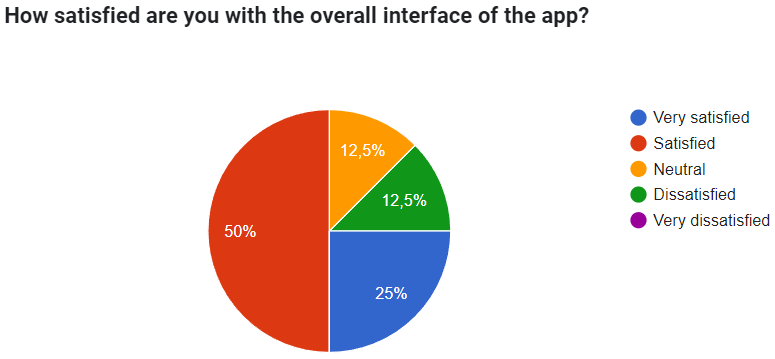
\includegraphics[width=0.9\linewidth]{figures/overall Interface.PNG}
    \caption{Results Overall Interface Impressions}
    \label{fig:overall interface}
\end{figure}

Figure \ref{fig:comments interface} shows the next question. Here the participants had the opportunity to make their own comments on the interface. This gives us a better understanding of the answers in the figure. On the one hand, the simplicity of the interface is mentioned here for the good ratings. The poor ratings can be explained by the nature of the prototype. This means that not all functions have been implemented yet and Figma does not always respond well in the browser application. What can be improved in the interface, however, is the understanding of the icons.
\begin{figure}[h!]
    \centering
    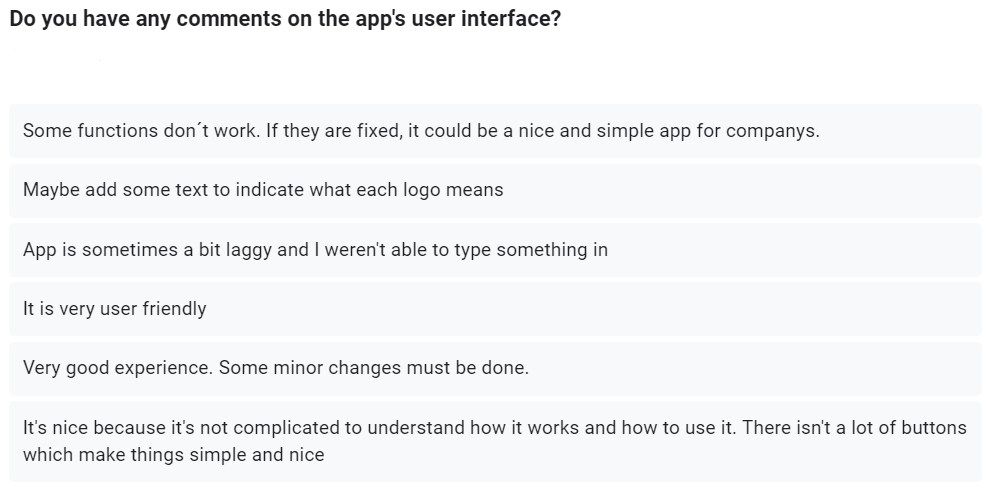
\includegraphics[width=0.9\linewidth]{figures/comments interface.PNG}
    \caption{Enter Caption}
    \label{fig:comments interface}
\end{figure}

As you can see in Figure \ref{fig:navigating}, we should think about whether the navigation between the screens can be handled more easily. 

\begin{figure}[h!]
    \centering
    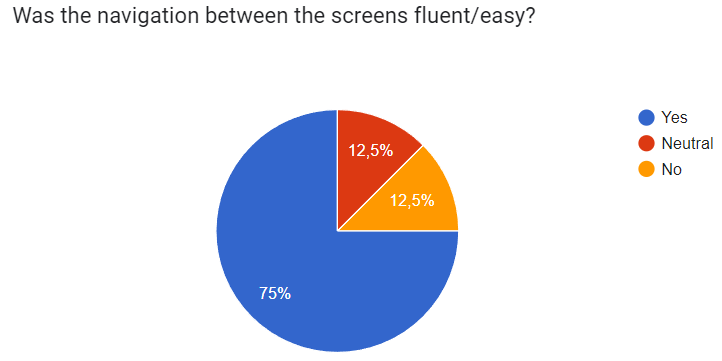
\includegraphics[width=0.8\linewidth]{figures/navigation easy.PNG}
    \caption{Nevigating between screens}
    \label{fig:navigating}
\end{figure}

\clearpage

\paragraph{Task-specific Feedback}\mbox{}\\
After the questions on general feedback, task-specific questions were asked. The first question asked was about creating a team, which, as can be seen in Figure \ref{fig:creating team}, was consistently perceived as easy.\\
\begin{figure}[h!]
    \centering
    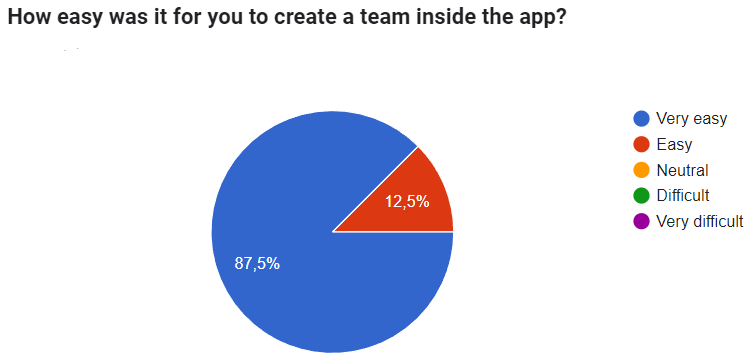
\includegraphics[width=0.8\linewidth]{figures/creating team.PNG}
    \caption{Creating a new team}
    \label{fig:creating team}
\end{figure}
As Figure \ref{fig:creating form} shows, creating a new survey was not quite as easy for the respondents.

\begin{figure}[h!]
    \centering
    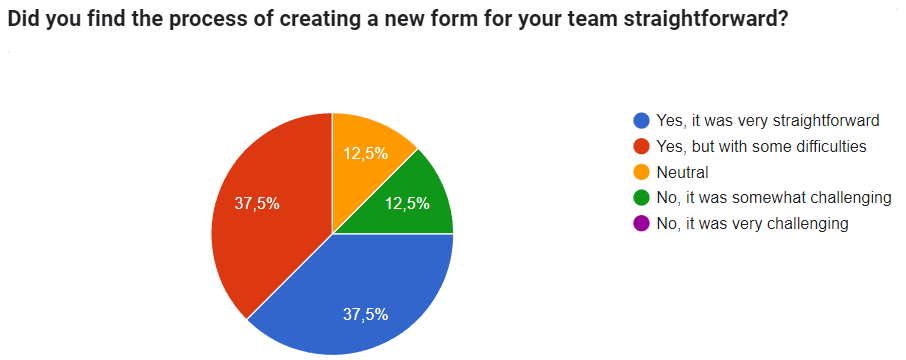
\includegraphics[width=0.9\linewidth]{figures/creating form.PNG}
    \caption{Creating a new form}
    \label{fig:creating form}
\end{figure}
The next question in Figure \ref{fig:comments form} can be used to explain the poorer results for creating the form. Here, the participants indicated the difficulties they had in creating a form. On the one hand, the problem of the prototype was noticed here again. Entering text is difficult with Figma, which is why this was ignored in our prototype. Secondly, the participants who found it difficult to create a new form found the selected icon unintuitive. A better, clearer solution should be considered here.
\begin{figure}[h!]
    \centering
    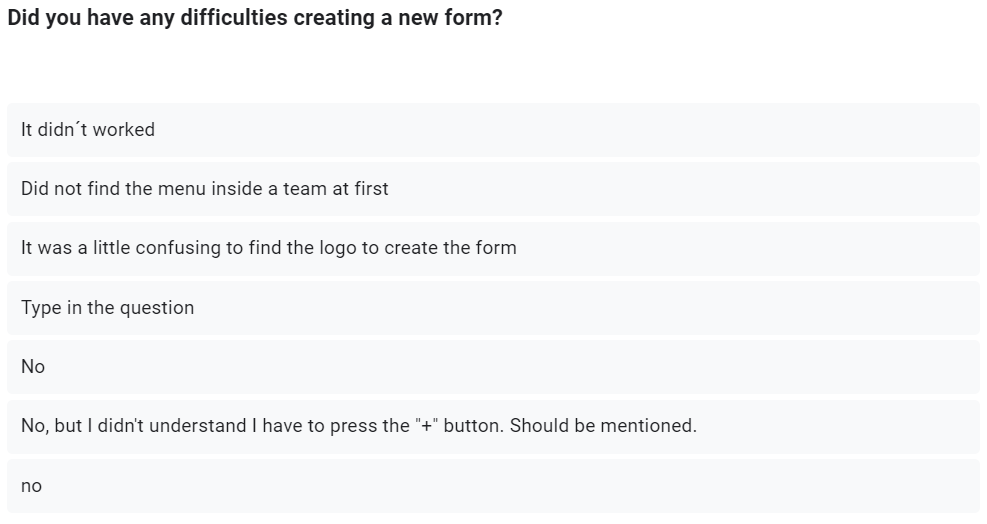
\includegraphics[width=0.9\linewidth]{figures/comments creating form.PNG}
    \caption{Enter Caption}
    \label{fig:comments form}
\end{figure}

\clearpage

\paragraph{Likability and Improvement} \mbox{}\\
In the last one, the participants were asked whether they would recommend the app to others. To our delight, there was no bad feedback here (Figure \ref{fig:recommend}).

\begin{figure}[h!]
    \centering
    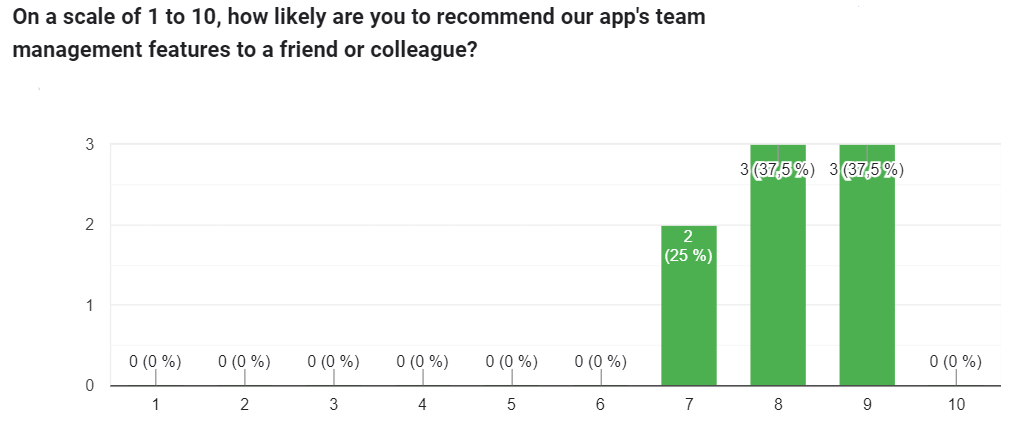
\includegraphics[width=0.9\linewidth]{figures/recommend.PNG}
    \caption{Probability of recommending the app}
    \label{fig:recommend}
\end{figure}
We then asked what the participants thought could be improved (Figure \ref{fig:comment improvement}). On the one hand, the task sheet was mentioned, which obviously left some uncertainties. On the other hand, the problems of the prototype, such as the text input, were mentioned again. As mentioned above, the choice of icons was also addressed again.
\begin{figure}[h!]
    \centering
    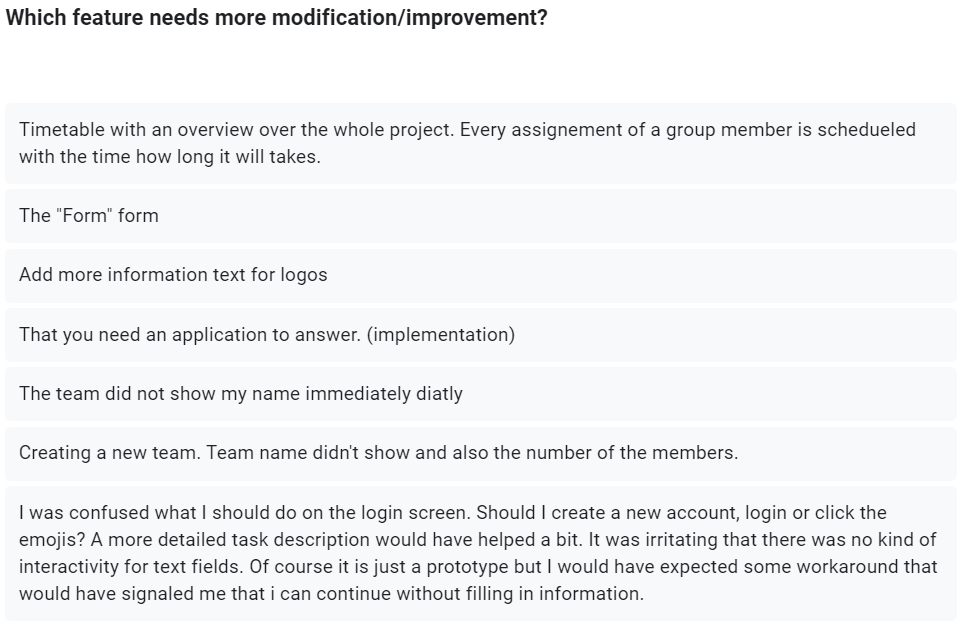
\includegraphics[width=0.9\linewidth]{figures/comments imrpovement needed.PNG}
    \caption{Enter Caption}
    \label{fig:comment improvement}
\end{figure}

Finally, the participants were given the opportunity to make their own comments on the app. The comments can be seen in Figure \ref{fig:general comments}.
\begin{figure}[h!]
    \centering
    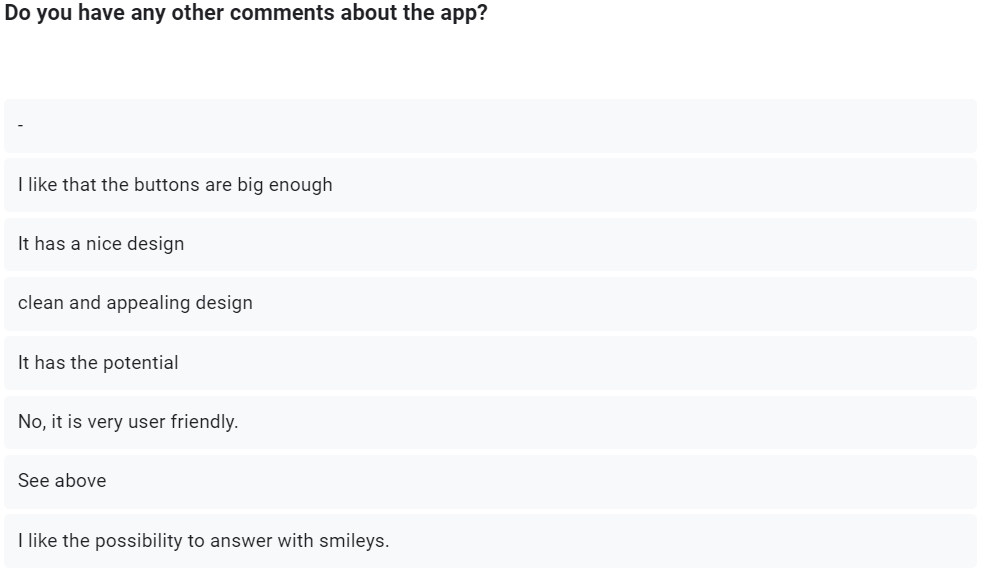
\includegraphics[width=0.9\linewidth]{figures/general comments.PNG}
    \caption{Enter Caption}
    \label{fig:general comments}
\end{figure}


\paragraph{Conclusion} \mbox{}\\
Overall, our participants had a really good experience by using our app, and we also got some pretty good feedback from them. The things that they mostly mentioned about future modification are the missing text of the logos (icons) of our app for better understanding. In addition, problems with the prototype were often mentioned that are not relevant for the final design but should be considered for the Hi-Fi prototype.\\
The idea was also raised to add a timetable with an overview of the entire project, in which the tasks of each team member are entered with a corresponding time limit. This is an aspect that could be considered for D4. Another point that did not appear in the surveys, but which was mentioned verbally by some participants, is the calendar with an overview of past daily moods. Some participants found this feature promising.\\

Here are some points we will be paying attention to in the future:
\begin{itemize}
    \item fix the problems with the prototype
    \item try to make the prototype as smooth and exact as possible
    \item improve the task descriptions for user tests
    \item adding some more text to the logos/icons or changing the icons
    \item improve the login screen
\end{itemize}



\section{Discussion}
All in all, the user tests have given us a good impression of what we still need to improve or which functions are already working well. We also realised that we should be a bit more precise in the task description to counteract the problem of the limited prototype. As text input with Figma, for example, is difficult, we should have specified default values here so that the user is not confused if the prototype displays different text than he has entered.\\
Looking at the Hi-Fi prototype, we now know better what we need to pay attention to in design and user testing and in which direction we need to develop.


% --------------------
\printbibliography

% ==========================
% ==========================
% ==========================


\end{document}